\documentclass[12pt,a4paper]{article}
\usepackage{amsmath, amssymb, geometry, booktabs, xcolor, hyperref,
            listings, pgfplots, tcolorbox, enumitem, fancyhdr, tikz, array}
\usepgfplotslibrary{fillbetween}
\geometry{margin=2.5cm}
\pgfplotsset{compat=1.18}
\tcbuselibrary{skins, breakable}

% Define custom environments
\newtcolorbox{curiositybox}[1]{colback=yellow!10, colframe=orange!80, title=#1, breakable}
\newtcolorbox{infobox}[1]{colback=blue!5, colframe=blue!60, title=#1, breakable}
\newtcolorbox{mistakebox}[1]{colback=red!5, colframe=red!60, title=#1, breakable}
\newtcolorbox{learnbox}[1]{colback=green!5, colframe=green!60, title=#1, breakable}

% Header and Footer
\pagestyle{fancy}
\fancyhf{}
\lhead{Eigenvalues and Eigenvectors}
\rhead{Unit 2 -- LAC}
\cfoot{\thepage}

% Document Title Setup
\title{\textbf{Eigenvalues and Eigenvectors} \\ \large Unit 2 -- Eigenvalues, Eigenvectors, Diagonalization and Quadratic Forms}
\author{Department of Mathematics}
\date{\today}

\begin{document}
\maketitle
\tableofcontents
\newpage

%============================================================
\section{Real-World Engineering Hook}
%============================================================

\begin{curiositybox}{Why Should an Engineer Care?}
In 1940, the Tacoma Narrows Bridge in Washington State catastrophically collapsed after only four months of service.
The culprit was not poor materials or faulty bolts --- it was \textbf{resonance}.
Every physical structure has \emph{natural frequencies}: the specific oscillation rates at which it vibrates
when disturbed. These natural frequencies are precisely the \textbf{eigenvalues} of the stiffness matrix
that encodes the structure's mechanical properties. The corresponding mode shapes --- the patterns in
which different parts of the structure move together --- are the \textbf{eigenvectors}.

When steady 42 km/h winds excited the bridge at a frequency matching one of its natural frequencies
(eigenvalue $\omega^2 \approx 0.2\,\text{rad}^2/\text{s}^2$), the amplitude grew without bound.
A civil engineer who had computed the eigenvalues of the bridge's stiffness matrix would have recognized
this danger and redesigned the deck cross-section.

\textbf{Beyond structural engineering:}
\begin{itemize}
  \item \textbf{Google PageRank} ranks every web page on the internet using the dominant eigenvector
        of a billion-by-billion link matrix. The most important page corresponds to the largest eigenvalue.
  \item \textbf{Principal Component Analysis (PCA)} in data science finds the eigenvectors of a
        covariance matrix to compress data while preserving maximum variance --- used in facial recognition,
        medical imaging, and financial risk modelling.
  \item \textbf{Quantum mechanics}: the energy levels of an atom are the eigenvalues of the Hamiltonian
        operator. Chemistry as we know it depends on eigenvalue theory.
\end{itemize}

Every time a building stands through an earthquake, a recommendation algorithm suggests your next video,
or an MRI scan produces a sharp image, eigenvalues and eigenvectors are working behind the scenes.
\end{curiositybox}

%============================================================
\section{Why This Topic Exists}
%============================================================

Eigenvalue theory transforms the study of linear transformations from abstract symbol manipulation
into a tool for predicting real physical behaviour.
Without eigenvalues we cannot determine whether a structure will resonate, whether an algorithm will
converge, or whether a dynamical system will remain stable.

\begin{center}
\begin{tabular}{@{}p{5.5cm} p{5.5cm} p{4cm}@{}}
\toprule
\textbf{Atomic Sub-Topic} & \textbf{Engineering Consequence} & \textbf{Typical Application} \\
\midrule
Definition of Eigenvalues and Eigenvectors &
  Identifies invariant directions of a system; structural mode shapes and natural frequencies &
  FEA, robotics \\
\addlinespace
Characteristic Equation and Polynomial &
  Characteristic roots of control-system transfer functions determine stability margins &
  Control engineering \\
\addlinespace
Finding Eigenvectors via Row Reduction &
  Computes mode shapes explicitly so engineers can design vibration dampers &
  Mechanical vibration \\
\addlinespace
Geometric vs Algebraic Multiplicity &
  Repeated eigenvalues with deficient eigenspaces signal non-diagonalizable (defective) systems &
  Coupled oscillators \\
\addlinespace
Eigenvalues of Special Matrices &
  Symmetric stiffness matrices guarantee real eigenvalues, ensuring real (physical) frequencies &
  Structural analysis \\
\bottomrule
\end{tabular}
\end{center}

\begin{learnbox}{Core Learning Objectives}
After studying this topic you will be able to:
\begin{enumerate}
  \item State and apply the definition $A\mathbf{x} = \lambda\mathbf{x}$.
  \item Form and solve the characteristic equation $\det(A - \lambda I) = 0$.
  \item Find eigenvectors by row-reducing $(A - \lambda I)\mathbf{x} = \mathbf{0}$.
  \item Distinguish algebraic and geometric multiplicity and state the inequality between them.
  \item Quote eigenvalue properties of triangular, symmetric, orthogonal, idempotent, and nilpotent matrices.
\end{enumerate}
\end{learnbox}

%============================================================
\section{Intuition and Mathematical Definitions}
%============================================================

%------------------------------------------------------------
\subsection{Definition of Eigenvalues and Eigenvectors}
%------------------------------------------------------------

Most vectors change both their \emph{direction} and \emph{length} when multiplied by a matrix.
Eigenvectors are special: they are the rare vectors that a matrix merely \emph{stretches or flips}
--- their direction is unchanged (or reversed), only their scale changes.
The scalar factor by which an eigenvector is scaled is called the eigenvalue.

Think of a rubber band stretched along the $x$-axis: any vector pointing along $x$ stays pointing along $x$;
it is an eigenvector. A vector pointing diagonally gets rotated --- it is not an eigenvector.

\begin{infobox}{Definition: Eigenvalue and Eigenvector}
Let $A$ be an $n \times n$ matrix. A scalar $\lambda$ is called an \textbf{eigenvalue} of $A$ if there
exists a \textbf{non-zero} vector $\mathbf{x} \in \mathbb{R}^n$ such that
\[
  A\mathbf{x} = \lambda\mathbf{x}.
\]
The non-zero vector $\mathbf{x}$ satisfying this equation is called an \textbf{eigenvector} of $A$
corresponding to $\lambda$.

\medskip
\textbf{Eigenspace:} The set of all solutions (including $\mathbf{0}$) to $(A - \lambda I)\mathbf{x} = \mathbf{0}$
forms a subspace of $\mathbb{R}^n$ called the \textbf{eigenspace} $E_\lambda$:
\[
  E_\lambda = \ker(A - \lambda I) = \{\mathbf{x} \mid (A - \lambda I)\mathbf{x} = \mathbf{0}\}.
\]

\textbf{Key facts:}
\begin{itemize}
  \item $\lambda = 0$ is a valid eigenvalue (iff $A$ is singular).
  \item The zero vector is \emph{never} an eigenvector by definition.
  \item If $\mathbf{x}$ is an eigenvector for $\lambda$, so is $c\mathbf{x}$ for any $c \neq 0$.
  \item The eigenspace $E_\lambda$ has dimension $\geq 1$.
\end{itemize}
\end{infobox}

\textbf{Worked Example 1.1 --- Verifying an eigenvalue/eigenvector pair.}

Let $A = \begin{pmatrix} 4 & 1 \\ 2 & 3 \end{pmatrix}$, $\lambda = 5$, $\mathbf{x} = \begin{pmatrix} 1 \\ 1 \end{pmatrix}$.

\textit{Step 1.} Compute $A\mathbf{x}$:
\[
  A\mathbf{x} = \begin{pmatrix} 4 & 1 \\ 2 & 3 \end{pmatrix}\begin{pmatrix} 1 \\ 1 \end{pmatrix}
  = \begin{pmatrix} 4(1)+1(1) \\ 2(1)+3(1) \end{pmatrix}
  = \begin{pmatrix} 5 \\ 5 \end{pmatrix}.
\]

\textit{Step 2.} Compute $\lambda\mathbf{x}$:
\[
  \lambda\mathbf{x} = 5\begin{pmatrix} 1 \\ 1 \end{pmatrix} = \begin{pmatrix} 5 \\ 5 \end{pmatrix}.
\]

\textit{Conclusion:} $A\mathbf{x} = \lambda\mathbf{x}$ is confirmed; $\lambda = 5$ is an eigenvalue
and $\mathbf{x} = \begin{pmatrix}1\\1\end{pmatrix}$ is a corresponding eigenvector.

%------------------------------------------------------------
\subsection{Characteristic Equation and Characteristic Polynomial}
%------------------------------------------------------------

To find \emph{all} eigenvalues of a matrix systematically, we rearrange $A\mathbf{x} = \lambda\mathbf{x}$
to $(A - \lambda I)\mathbf{x} = \mathbf{0}$. For this to have a non-zero solution, the matrix
$(A - \lambda I)$ must be singular --- its determinant must be zero.
This determinant, viewed as a function of $\lambda$, is a polynomial whose roots are exactly the eigenvalues.

\begin{infobox}{Characteristic Polynomial and Characteristic Equation}
The \textbf{characteristic polynomial} of an $n \times n$ matrix $A$ is
\[
  p(\lambda) = \det(A - \lambda I).
\]
\begin{itemize}
  \item $p(\lambda)$ is a polynomial of degree $n$ in $\lambda$.
  \item The leading term is $(-1)^n \lambda^n$ for the standard convention $\det(A - \lambda I)$
        (some texts use $\det(\lambda I - A)$, giving leading term $+\lambda^n$; both give the same roots).
  \item The \textbf{characteristic equation} is $p(\lambda) = 0$, i.e.\ $\det(A - \lambda I) = 0$.
  \item The roots of $p(\lambda) = 0$ are the eigenvalues of $A$ (possibly complex, possibly repeated).
  \item $\text{trace}(A) = \sum_{i=1}^n \lambda_i$ and $\det(A) = \prod_{i=1}^n \lambda_i$
        (counting multiplicity).
\end{itemize}
\end{infobox}

\textbf{Worked Example 2.1 --- Computing the characteristic polynomial.}

Let $B = \begin{pmatrix} 3 & -2 \\ 1 & 0 \end{pmatrix}$.

\textit{Step 1.} Form $B - \lambda I$:
\[
  B - \lambda I = \begin{pmatrix} 3-\lambda & -2 \\ 1 & -\lambda \end{pmatrix}.
\]

\textit{Step 2.} Compute the determinant:
\[
  p(\lambda) = \det\begin{pmatrix} 3-\lambda & -2 \\ 1 & -\lambda \end{pmatrix}
  = (3-\lambda)(-\lambda) - (-2)(1)
  = -3\lambda + \lambda^2 + 2
  = \lambda^2 - 3\lambda + 2.
\]

\textit{Step 3.} Factor:
\[
  p(\lambda) = (\lambda - 1)(\lambda - 2).
\]

\textit{Eigenvalues:} $\lambda_1 = 1$, $\lambda_2 = 2$.

\textit{Verification using trace and determinant:}
$\lambda_1 + \lambda_2 = 1 + 2 = 3 = \text{trace}(B)$ \checkmark; \quad
$\lambda_1 \cdot \lambda_2 = 1 \times 2 = 2 = \det(B) = (3)(0) - (-2)(1) = 2$ \checkmark.

%------------------------------------------------------------
\subsection{Finding Eigenvectors via Row Reduction}
%------------------------------------------------------------

Once we know an eigenvalue $\lambda_k$, we substitute it back into $(A - \lambda_k I)\mathbf{x} = \mathbf{0}$
and solve the homogeneous system. The system is guaranteed to be under-determined (rank deficient),
so it always has infinitely many solutions. Row reduction reveals the free variables and expresses the
general solution --- the \emph{eigenspace basis}.

\begin{infobox}{Procedure: Eigenvector Calculation by Row Reduction}
\textbf{Given:} eigenvalue $\lambda_k$ of $A$ (an $n\times n$ matrix).

\textbf{Step 1.} Form $M = A - \lambda_k I$.

\textbf{Step 2.} Augment: $[M \mid \mathbf{0}]$ and row-reduce to reduced row echelon form (RREF).

\textbf{Step 3.} Identify \emph{free variables} (columns without pivots).

\textbf{Step 4.} Express pivot variables in terms of free variables.

\textbf{Step 5.} Assign parameter values (e.g.\ $t=1$) to free variables and write
the \textbf{eigenvector basis} for $E_{\lambda_k}$.

\textbf{Note:} $\dim(E_{\lambda_k}) = n - \text{rank}(A - \lambda_k I)$.
\end{infobox}

\textbf{Worked Example 3.1 --- Eigenvectors of a $2\times 2$ matrix.}

Using $B = \begin{pmatrix} 3 & -2 \\ 1 & 0 \end{pmatrix}$ from Example 2.1 with eigenvalues $\lambda_1 = 1$, $\lambda_2 = 2$.

\textbf{For $\lambda_1 = 1$:}

\textit{Step 1.} $B - I = \begin{pmatrix} 2 & -2 \\ 1 & -1 \end{pmatrix}$.

\textit{Step 2.} Row reduce:
\[
  \begin{pmatrix} 2 & -2 \\ 1 & -1 \end{pmatrix}
  \xrightarrow{R_1 \leftarrow R_1/2}
  \begin{pmatrix} 1 & -1 \\ 1 & -1 \end{pmatrix}
  \xrightarrow{R_2 \leftarrow R_2 - R_1}
  \begin{pmatrix} 1 & -1 \\ 0 & 0 \end{pmatrix}.
\]

\textit{Step 3.} Equation: $x_1 - x_2 = 0$, so $x_1 = x_2$. Let $x_2 = t$.

\textit{Step 4.} Eigenvector: $\mathbf{x} = t\begin{pmatrix} 1 \\ 1 \end{pmatrix}$. Basis: $\left\{\begin{pmatrix}1\\1\end{pmatrix}\right\}$.

\textbf{For $\lambda_2 = 2$:}

\textit{Step 1.} $B - 2I = \begin{pmatrix} 1 & -2 \\ 1 & -2 \end{pmatrix}$.

\textit{Step 2.} Row reduce:
\[
  \begin{pmatrix} 1 & -2 \\ 1 & -2 \end{pmatrix}
  \xrightarrow{R_2 \leftarrow R_2 - R_1}
  \begin{pmatrix} 1 & -2 \\ 0 & 0 \end{pmatrix}.
\]

\textit{Step 3.} Equation: $x_1 = 2x_2$. Let $x_2 = s$.

\textit{Step 4.} Eigenvector: $\mathbf{x} = s\begin{pmatrix} 2 \\ 1 \end{pmatrix}$. Basis: $\left\{\begin{pmatrix}2\\1\end{pmatrix}\right\}$.

%------------------------------------------------------------
\subsection{Geometric vs Algebraic Multiplicity}
%------------------------------------------------------------

When the characteristic polynomial has a repeated root, the eigenvalue's root-multiplicity (algebraic)
and its eigenspace dimension (geometric) may or may not agree.
This distinction determines whether a matrix is diagonalizable --- a critical property for
computing matrix powers and solving differential equations.

\begin{infobox}{Algebraic and Geometric Multiplicity}
Let $\lambda_k$ be an eigenvalue of $A$.

\begin{itemize}
  \item \textbf{Algebraic multiplicity} $m_a(\lambda_k)$: the multiplicity of $\lambda_k$ as a root
        of the characteristic polynomial $p(\lambda)$.
  \item \textbf{Geometric multiplicity} $m_g(\lambda_k)$: the dimension of the eigenspace $E_{\lambda_k}$,
        i.e.\ $m_g(\lambda_k) = \dim\ker(A - \lambda_k I) = n - \text{rank}(A - \lambda_k I)$.
\end{itemize}

\textbf{Fundamental inequality:}
\[
  1 \leq m_g(\lambda_k) \leq m_a(\lambda_k).
\]

\textbf{Diagonalizability criterion:} $A$ is diagonalizable if and only if
$m_g(\lambda_k) = m_a(\lambda_k)$ for \emph{every} eigenvalue $\lambda_k$.

When $m_g < m_a$ for some eigenvalue, the matrix is called \textbf{defective}.
\end{infobox}

\textbf{Worked Example 4.1 --- Defective matrix (multiplicities differ).}

Let $C = \begin{pmatrix} 5 & 1 \\ 0 & 5 \end{pmatrix}$.

\textit{Step 1. Characteristic polynomial:}
\[
  p(\lambda) = \det\begin{pmatrix} 5-\lambda & 1 \\ 0 & 5-\lambda \end{pmatrix}
  = (5-\lambda)^2.
\]
So $\lambda = 5$ is the only eigenvalue, with $m_a(5) = 2$.

\textit{Step 2. Eigenvectors for $\lambda = 5$:}
\[
  C - 5I = \begin{pmatrix} 0 & 1 \\ 0 & 0 \end{pmatrix}.
\]
Row form is already in RREF. Equation: $x_2 = 0$; $x_1$ is free.
Eigenvector: $\mathbf{x} = t\begin{pmatrix}1\\0\end{pmatrix}$.

\textit{Step 3. Multiplicities:}
$m_g(5) = \dim E_5 = 1$, but $m_a(5) = 2$.

Since $m_g(5) = 1 < 2 = m_a(5)$, matrix $C$ is \textbf{defective} and \emph{not} diagonalizable.

%------------------------------------------------------------
\subsection{Eigenvalues of Special Matrices}
%------------------------------------------------------------

Certain structural properties of a matrix directly constrain its eigenvalues.
Knowing these results saves computation and builds intuition.
A symmetric stiffness matrix is guaranteed to have real eigenvalues --- this means
the natural frequencies of a physical structure are always real numbers, which is physically sensible.

\begin{infobox}{Eigenvalue Properties of Special Matrices}
\begin{enumerate}
  \item \textbf{Triangular matrix} (upper or lower):
        The eigenvalues are the \emph{diagonal entries}. \\
        If $A$ is triangular, $p(\lambda) = \prod_{i=1}^n (a_{ii} - \lambda)$.

  \item \textbf{Symmetric matrix} ($A = A^T$, real entries):
        All eigenvalues are \emph{real}. Eigenvectors corresponding to distinct eigenvalues
        are orthogonal.

  \item \textbf{Orthogonal matrix} ($A^T A = I$):
        Every eigenvalue satisfies $|\lambda| = 1$.
        Real eigenvalues can only be $\pm 1$.

  \item \textbf{Idempotent matrix} ($A^2 = A$):
        Every eigenvalue is either $0$ or $1$.
        (Proof: $A\mathbf{x}=\lambda\mathbf{x} \Rightarrow A^2\mathbf{x}=\lambda^2\mathbf{x}=\lambda\mathbf{x} \Rightarrow \lambda(\lambda-1)=0$.)

  \item \textbf{Nilpotent matrix} ($A^k = 0$ for some positive integer $k$):
        All eigenvalues are $0$.
        (Proof: $A^k\mathbf{x}=\lambda^k\mathbf{x}=\mathbf{0} \Rightarrow \lambda^k=0 \Rightarrow \lambda=0$.)
\end{enumerate}
\end{infobox}

\textbf{Worked Example 5.1 --- Eigenvalues of a lower triangular matrix by inspection.}

Let $T = \begin{pmatrix} 2 & 0 & 0 \\ 3 & -1 & 0 \\ 7 & 4 & 6 \end{pmatrix}$.

Since $T$ is lower triangular, its eigenvalues are the diagonal entries:
\[
  \lambda_1 = 2, \quad \lambda_2 = -1, \quad \lambda_3 = 6.
\]

\textit{Verification via characteristic polynomial:}
\[
  p(\lambda) = \det(T - \lambda I)
  = (2-\lambda)(-1-\lambda)(6-\lambda).
\]
Roots are $\lambda = 2, -1, 6$ --- confirming the diagonal entries. \checkmark

%============================================================
\section{Visual Artifacts and Geometric Interpretation}
%============================================================

\subsection*{Diagram 1: Eigenvector direction preserved under matrix transformation}

The following TikZ diagram shows how a general vector $\mathbf{v}$ gets rotated by $A$,
while an eigenvector $\mathbf{x}$ only gets scaled (its direction is preserved).

\begin{center}
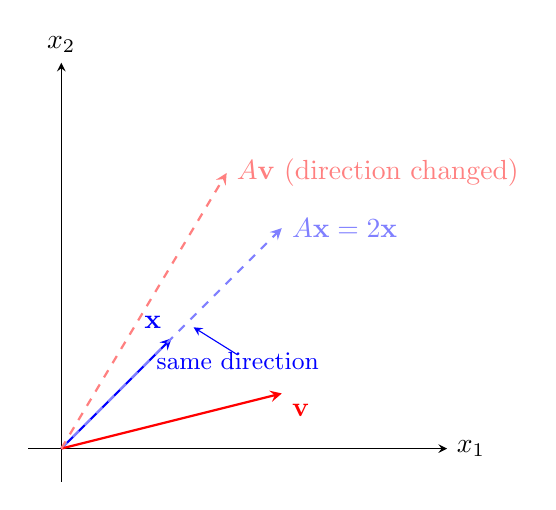
\begin{tikzpicture}[scale=1.4, >=stealth]
  % Axes
  \draw[->] (-0.3,0) -- (3.5,0) node[right] {$x_1$};
  \draw[->] (0,-0.3) -- (0,3.5) node[above] {$x_2$};
  % Original eigenvector
  \draw[->, thick, blue] (0,0) -- (1,1) node[above left] {$\mathbf{x}$};
  % Scaled eigenvector A*x = lambda*x (lambda=2)
  \draw[->, thick, blue!50, dashed] (0,0) -- (2,2) node[right] {$A\mathbf{x} = 2\mathbf{x}$};
  % Non-eigenvector
  \draw[->, thick, red] (0,0) -- (2,0.5) node[below right] {$\mathbf{v}$};
  % Transformed non-eigenvector (rotated and scaled)
  \draw[->, thick, red!50, dashed] (0,0) -- (1.5,2.5) node[right] {$A\mathbf{v}$ (direction changed)};
  % Labels
  \node[blue] at (1.6,0.8) {\small same direction};
  \draw[blue, ->] (1.6,0.85) -- (1.2,1.1);
\end{tikzpicture}
\end{center}

\subsection*{Diagram 2: Characteristic polynomial $p(\lambda)$ vs $\lambda$}

For $B = \begin{pmatrix}3&-2\\1&0\end{pmatrix}$, the characteristic polynomial is $p(\lambda)=\lambda^2-3\lambda+2$.
The roots $\lambda=1$ and $\lambda=2$ are the eigenvalues.

\begin{center}
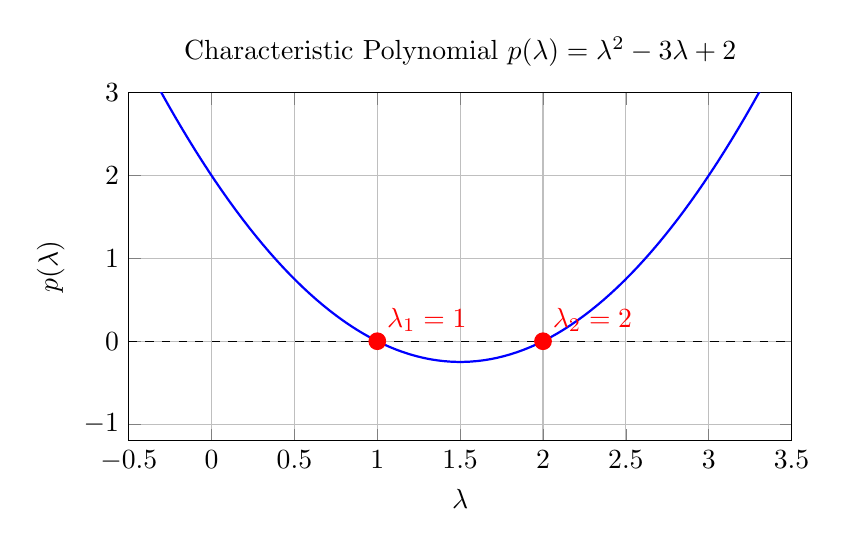
\begin{tikzpicture}
\begin{axis}[
  xlabel={$\lambda$},
  ylabel={$p(\lambda)$},
  xmin=-0.5, xmax=3.5,
  ymin=-1.2, ymax=3,
  samples=100,
  grid=both,
  width=10cm, height=6cm,
  title={Characteristic Polynomial $p(\lambda)=\lambda^2-3\lambda+2$}
]
  \addplot[blue, thick, domain=-0.5:3.5] {x^2 - 3*x + 2};
  \addplot[only marks, mark=*, mark size=3pt, red]
    coordinates {(1,0) (2,0)};
  \node[red, above right] at (axis cs:1,0) {$\lambda_1=1$};
  \node[red, above right] at (axis cs:2,0) {$\lambda_2=2$};
  \addplot[black, dashed, domain=-0.5:3.5] {0};
\end{axis}
\end{tikzpicture}
\end{center}

\subsection*{Diagram 3: Geometric vs Algebraic Multiplicity (Eigenspace dimension)}

\begin{center}
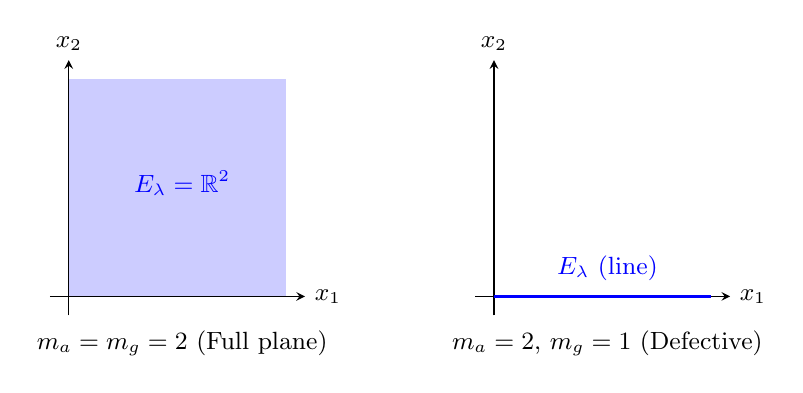
\begin{tikzpicture}[scale=1.2, >=stealth]
  % Left: full 2D eigenspace (alg=geo=2)
  \begin{scope}[xshift=0cm]
    \draw[->] (-0.2,0)--(2.5,0) node[right]{\small $x_1$};
    \draw[->] (0,-0.2)--(0,2.5) node[above]{\small $x_2$};
    \fill[blue!20] (0,0) -- (2.3,0) -- (2.3,2.3) -- (0,2.3) -- cycle;
    \node[blue] at (1.2,1.2) {\small $E_\lambda = \mathbb{R}^2$};
    \node at (1.2,-0.5) {\small $m_a=m_g=2$ (Full plane)};
  \end{scope}
  % Right: 1D eigenspace (geo=1 < alg=2, defective)
  \begin{scope}[xshift=4.5cm]
    \draw[->] (-0.2,0)--(2.5,0) node[right]{\small $x_1$};
    \draw[->] (0,-0.2)--(0,2.5) node[above]{\small $x_2$};
    \draw[blue, very thick] (0,0) -- (2.3,0);
    \node[blue] at (1.2,0.3) {\small $E_\lambda$ (line)};
    \node at (1.2,-0.5) {\small $m_a=2$, $m_g=1$ (Defective)};
  \end{scope}
\end{tikzpicture}
\end{center}

%============================================================
\section{Step-by-Step Algorithmic Workflow}
%============================================================

\begin{infobox}{Algorithm: Computing Eigenvalues and Eigenvectors of an $n\times n$ Matrix}
\textbf{Input:} Square matrix $A$ of order $n$.\\
\textbf{Output:} All eigenvalues $\lambda_i$ and corresponding eigenvector bases.

\medskip
\textbf{Step 1: Form $A - \lambda I$.}\\
Subtract $\lambda$ from each diagonal entry of $A$.

\medskip
\textbf{Step 2: Compute the characteristic polynomial.}\\
Evaluate $p(\lambda) = \det(A - \lambda I)$. For a $2\times 2$ matrix:
\[
  p(\lambda) = (a_{11}-\lambda)(a_{22}-\lambda) - a_{12}a_{21}.
\]
For larger matrices, use cofactor expansion along a convenient row or column.

\medskip
\textbf{Step 3: Solve the characteristic equation.}\\
Set $p(\lambda) = 0$ and solve for all roots $\lambda_1, \lambda_2, \ldots, \lambda_k$ (counting multiplicity).
Factor the polynomial algebraically. For cubics and quartics, try rational roots first.

\medskip
\textbf{Step 4: Find eigenvectors for each eigenvalue.}\\
For each distinct eigenvalue $\lambda_i$:
\begin{enumerate}[(a)]
  \item Substitute $\lambda_i$ into $A - \lambda_i I$.
  \item Row-reduce $[A - \lambda_i I \mid \mathbf{0}]$ to RREF.
  \item Identify free variables (columns without leading 1s).
  \item Express pivot variables in terms of free variables.
  \item Assign $t = 1$ (or $t=1, s=0$ and $t=0, s=1$ for two free variables) to generate basis vectors.
\end{enumerate}

\medskip
\textbf{Step 5: State the eigenspace basis.}\\
Write $E_{\lambda_i} = \text{span}\{\mathbf{v}_1, \mathbf{v}_2, \ldots\}$ for the vectors obtained in Step 4.

\medskip
\textbf{Step 6: Check multiplicities (optional but recommended).}\\
Confirm $m_g(\lambda_i) = $ number of basis vectors found; compare with $m_a(\lambda_i)$ from Step 3.
\end{infobox}

%============================================================
\section{Fully Worked Numerical Examples}
%============================================================

\subsection*{Example 6.1 --- $2\times 2$ matrix: find eigenvalues, eigenvectors, verify $A\mathbf{x}=\lambda\mathbf{x}$}

Let $A = \begin{pmatrix} 6 & 2 \\ 2 & 3 \end{pmatrix}$.

\textbf{Step 1.} Form $A - \lambda I$:
\[
  A - \lambda I = \begin{pmatrix} 6-\lambda & 2 \\ 2 & 3-\lambda \end{pmatrix}.
\]

\textbf{Step 2.} Characteristic polynomial:
\[
  p(\lambda) = (6-\lambda)(3-\lambda) - (2)(2)
  = 18 - 6\lambda - 3\lambda + \lambda^2 - 4
  = \lambda^2 - 9\lambda + 14.
\]

\textbf{Step 3.} Solve $\lambda^2 - 9\lambda + 14 = 0$:
\[
  (\lambda - 7)(\lambda - 2) = 0 \implies \lambda_1 = 7,\quad \lambda_2 = 2.
\]

\textbf{Step 4. Eigenvector for $\lambda_1 = 7$:}
\[
  A - 7I = \begin{pmatrix} -1 & 2 \\ 2 & -4 \end{pmatrix}
  \xrightarrow{R_2 \leftarrow R_2 + 2R_1}
  \begin{pmatrix} -1 & 2 \\ 0 & 0 \end{pmatrix}
  \xrightarrow{R_1 \leftarrow -R_1}
  \begin{pmatrix} 1 & -2 \\ 0 & 0 \end{pmatrix}.
\]
Equation: $x_1 = 2x_2$. Let $x_2 = 1$: $\mathbf{x}_1 = \begin{pmatrix}2\\1\end{pmatrix}$.

\textbf{Step 5. Eigenvector for $\lambda_2 = 2$:}
\[
  A - 2I = \begin{pmatrix} 4 & 2 \\ 2 & 1 \end{pmatrix}
  \xrightarrow{R_2 \leftarrow R_2 - \frac{1}{2}R_1}
  \begin{pmatrix} 4 & 2 \\ 0 & 0 \end{pmatrix}
  \xrightarrow{R_1 \leftarrow R_1/4}
  \begin{pmatrix} 1 & 1/2 \\ 0 & 0 \end{pmatrix}.
\]
Equation: $x_1 = -\tfrac{1}{2}x_2$. Let $x_2 = 2$: $\mathbf{x}_2 = \begin{pmatrix}-1\\2\end{pmatrix}$.

\textbf{Step 6. Verification ($\lambda_1 = 7$):}
\[
  A\mathbf{x}_1 = \begin{pmatrix}6&2\\2&3\end{pmatrix}\begin{pmatrix}2\\1\end{pmatrix}
  = \begin{pmatrix}12+2\\4+3\end{pmatrix} = \begin{pmatrix}14\\7\end{pmatrix}
  = 7\begin{pmatrix}2\\1\end{pmatrix} = \lambda_1\mathbf{x}_1. \checkmark
\]

\subsection*{Example 6.2 --- $3\times 3$ triangular matrix: eigenvalues by inspection, eigenvectors by row reduction}

Let $D = \begin{pmatrix} 4 & 5 & 6 \\ 0 & 3 & 1 \\ 0 & 0 & -2 \end{pmatrix}$.

\textbf{Step 1. Eigenvalues by inspection} (upper triangular):
\[
  \lambda_1 = 4,\quad \lambda_2 = 3,\quad \lambda_3 = -2.
\]
All distinct, so $m_a = m_g = 1$ for each.

\textbf{Step 2. Eigenvector for $\lambda_1 = 4$:}
\[
  D - 4I = \begin{pmatrix} 0 & 5 & 6 \\ 0 & -1 & 1 \\ 0 & 0 & -6 \end{pmatrix}.
\]
Augment with zero column and row reduce:
\[
  \begin{pmatrix} 0&5&6\\0&-1&1\\0&0&-6 \end{pmatrix}
  \xrightarrow{R_3\leftarrow R_3/(-6)}
  \begin{pmatrix}0&5&6\\0&-1&1\\0&0&1\end{pmatrix}
  \xrightarrow{R_2\leftarrow R_2-R_3}
  \begin{pmatrix}0&5&6\\0&-1&0\\0&0&1\end{pmatrix}
  \xrightarrow{R_2\leftarrow-R_2}
  \begin{pmatrix}0&5&6\\0&1&0\\0&0&1\end{pmatrix}.
\]
\[
  \xrightarrow{R_1\leftarrow R_1-6R_3}
  \begin{pmatrix}0&5&0\\0&1&0\\0&0&1\end{pmatrix}
  \xrightarrow{R_1\leftarrow R_1-5R_2}
  \begin{pmatrix}0&0&0\\0&1&0\\0&0&1\end{pmatrix}.
\]
$x_1$ is free; set $x_1=1$: $\mathbf{x}_1=\begin{pmatrix}1\\0\\0\end{pmatrix}$.

\textbf{Step 3. Eigenvector for $\lambda_2 = 3$:}
\[
  D-3I = \begin{pmatrix}1&5&6\\0&0&1\\0&0&-5\end{pmatrix}
  \xrightarrow{R_3\leftarrow R_3+5R_2}
  \begin{pmatrix}1&5&6\\0&0&1\\0&0&0\end{pmatrix}
  \xrightarrow{R_1\leftarrow R_1-6R_2}
  \begin{pmatrix}1&5&0\\0&0&1\\0&0&0\end{pmatrix}.
\]
$x_2$ free; set $x_2=1$: $x_1=-5$, $x_3=0$. $\mathbf{x}_2=\begin{pmatrix}-5\\1\\0\end{pmatrix}$.

\textbf{Step 4. Eigenvector for $\lambda_3 = -2$:}
\[
  D+2I = \begin{pmatrix}6&5&6\\0&5&1\\0&0&0\end{pmatrix}.
\]
Row reduce:
\[
  \xrightarrow{R_2\leftarrow R_2/5}
  \begin{pmatrix}6&5&6\\0&1&1/5\\0&0&0\end{pmatrix}
  \xrightarrow{R_1\leftarrow R_1-5R_2}
  \begin{pmatrix}6&0&5\\0&1&1/5\\0&0&0\end{pmatrix}
  \xrightarrow{R_1\leftarrow R_1/6}
  \begin{pmatrix}1&0&5/6\\0&1&1/5\\0&0&0\end{pmatrix}.
\]
$x_3$ free; set $x_3=30$: $x_1=-25$, $x_2=-6$. $\mathbf{x}_3=\begin{pmatrix}-25\\-6\\30\end{pmatrix}$.

\subsection*{Example 6.3 --- Engineering: Vibration of a 2-DOF spring-mass system}

\textbf{Problem setup.} Two masses $m_1 = m_2 = 1\,\text{kg}$ are connected by three springs with
stiffness $k_1 = k_3 = 2\,\text{N/m}$ (outer) and $k_2 = 1\,\text{N/m}$ (coupling spring).
The stiffness matrix is
\[
  K = \begin{pmatrix} k_1+k_2 & -k_2 \\ -k_2 & k_2+k_3 \end{pmatrix}
    = \begin{pmatrix} 3 & -1 \\ -1 & 3 \end{pmatrix}.
\]
The mass matrix is $M = I_2$ (identity, since both masses equal 1).
Equation of motion: $M\ddot{\mathbf{u}} + K\mathbf{u} = \mathbf{0}$, giving eigenvalue problem $K\mathbf{x}=\omega^2\mathbf{x}$.

\textbf{Step 1.} Characteristic polynomial:
\[
  \det(K - \omega^2 I)
  = \det\begin{pmatrix}3-\omega^2 & -1 \\ -1 & 3-\omega^2\end{pmatrix}
  = (3-\omega^2)^2 - 1
  = \omega^4 - 6\omega^2 + 9 - 1
  = \omega^4 - 6\omega^2 + 8.
\]

\textbf{Step 2.} Let $\mu = \omega^2$: $\mu^2 - 6\mu + 8 = (\mu-2)(\mu-4) = 0$.
So $\mu_1 = 2$, $\mu_2 = 4$.

\textbf{Step 3.} Natural frequencies: $\omega_1 = \sqrt{2}\,\text{rad/s}$, $\omega_2 = 2\,\text{rad/s}$.

\textbf{Step 4. Mode shape for $\mu_1 = 2$:}
\[
  K - 2I = \begin{pmatrix}1&-1\\-1&1\end{pmatrix}
  \xrightarrow{R_2\leftarrow R_2+R_1}
  \begin{pmatrix}1&-1\\0&0\end{pmatrix}.
\]
$x_1 = x_2$. Mode shape: $\mathbf{x}_1 = \begin{pmatrix}1\\1\end{pmatrix}$ --- \emph{in-phase} mode (both masses move together).

\textbf{Step 5. Mode shape for $\mu_2 = 4$:}
\[
  K - 4I = \begin{pmatrix}-1&-1\\-1&-1\end{pmatrix}
  \xrightarrow{R_2\leftarrow R_2-R_1}
  \begin{pmatrix}-1&-1\\0&0\end{pmatrix}
  \xrightarrow{R_1\leftarrow -R_1}
  \begin{pmatrix}1&1\\0&0\end{pmatrix}.
\]
$x_1 = -x_2$. Mode shape: $\mathbf{x}_2 = \begin{pmatrix}1\\-1\end{pmatrix}$ --- \emph{out-of-phase} mode (masses move oppositely).

\textbf{Physical interpretation:} At $\omega_1=\sqrt{2}$ rad/s the two masses oscillate together; at $\omega_2=2$ rad/s they
oscillate in opposition. An engineer designing vibration isolation must ensure external excitation frequencies
avoid both $\sqrt{2}$ and $2$ rad/s.

%============================================================
\section{Tabular Reference}
%============================================================

\begin{center}
\begin{tabular}{@{}p{3cm} p{5cm} p{4cm} p{3.5cm}@{}}
\toprule
\textbf{Property} & \textbf{Algebraic Multiplicity $m_a$} & \textbf{Geometric Multiplicity $m_g$} & \textbf{Implication} \\
\midrule
Definition &
  Multiplicity of $\lambda$ as a root of $p(\lambda)=\det(A-\lambda I)$ &
  $\dim\ker(A-\lambda I) = n-\text{rank}(A-\lambda I)$ &
  ---\\
\addlinespace
Relation &
  $m_a \geq 1$ always &
  $1 \leq m_g \leq m_a$ &
  $m_g$ cannot exceed $m_a$ \\
\addlinespace
Equal case ($m_g=m_a$) &
  $A$ has a full eigenspace for $\lambda$ &
  Eigenspace has basis of $m_a$ vectors &
  $A$ is \textbf{diagonalizable} \\
\addlinespace
Unequal case ($m_g < m_a$) &
  $\lambda$ appears multiple times as root &
  Eigenspace is ``too small'' &
  $A$ is \textbf{defective}; Jordan form needed \\
\addlinespace
Example ($m_a=m_g$) &
  $\lambda=2$ with $m_a=2$ for $A=2I$ &
  $E_2=\mathbb{R}^2$, $m_g=2$ &
  Diagonalizable \\
\addlinespace
Example ($m_a>m_g$) &
  $\lambda=5$ with $m_a=2$ for $\begin{pmatrix}5&1\\0&5\end{pmatrix}$ &
  $m_g=1$ (only $\begin{pmatrix}1\\0\end{pmatrix}$) &
  Defective \\
\bottomrule
\end{tabular}
\end{center}

%============================================================
\section{Common Student Mistakes and Pitfalls}
%============================================================

\begin{mistakebox}{Common Mistakes in Eigenvalue Problems}
\begin{tabular}{@{}p{4cm} p{5cm} p{5cm}@{}}
\toprule
\textbf{Sub-Topic} & \textbf{Mistake} & \textbf{Correction} \\
\midrule
Definition &
  Accepting $\mathbf{x}=\mathbf{0}$ as an eigenvector &
  By definition, eigenvectors must be \emph{non-zero}; $\mathbf{0}$ is excluded \\
\addlinespace
Definition &
  Confusing the eigenvalue equation as $A\mathbf{x}=\lambda$ (scalar) &
  The equation is $A\mathbf{x}=\lambda\mathbf{x}$; $\lambda$ multiplies the vector $\mathbf{x}$ \\
\addlinespace
Characteristic Polynomial &
  Forgetting the $-\lambda$ on \emph{all} diagonal entries &
  $A-\lambda I$ subtracts $\lambda$ from \emph{every} diagonal entry $a_{ii}$, not just $a_{11}$ \\
\addlinespace
Characteristic Polynomial &
  Sign error: computing $\det(\lambda I - A)$ vs $\det(A - \lambda I)$ &
  Both give the same roots; choose one convention and apply it consistently \\
\addlinespace
Row Reduction for Eigenvectors &
  Row reducing $A-\lambda I$ and then using the \emph{augmented} rows as eigenvectors &
  Row-reduce the \emph{homogeneous} system; eigenvectors come from the \emph{null space}, not the row space \\
\addlinespace
Row Reduction &
  Stopping row reduction too early and missing a free variable &
  Always reduce to full RREF; check that rank $= n - (\text{number of free variables})$ \\
\addlinespace
Geometric vs Algebraic Multiplicity &
  Assuming $m_g = m_a$ always &
  This holds for real symmetric matrices but not in general; check with a defective example \\
\addlinespace
Geometric vs Algebraic Multiplicity &
  Claiming a matrix with a repeated eigenvalue is always non-diagonalizable &
  A repeated eigenvalue with $m_g=m_a$ (e.g.\ $A=5I$) is still diagonalizable \\
\addlinespace
Special Matrices &
  Claiming a non-diagonal triangular matrix has only one eigenvalue &
  A triangular matrix has \emph{all} diagonal entries as eigenvalues, which may be distinct \\
\addlinespace
Special Matrices &
  Assuming real symmetric matrices can have complex eigenvalues &
  Real symmetric matrices are guaranteed to have only \emph{real} eigenvalues \\
\bottomrule
\end{tabular}
\end{mistakebox}

%============================================================
\section{Comprehensive Assessment Suite}
%============================================================

\subsection*{Viva-Voce Questions}

\begin{enumerate}
  \item \textbf{(Sub-topic 1)} State the definition of an eigenvalue and eigenvector of a matrix $A$.
        Why must the eigenvector be non-zero?
  \item \textbf{(Sub-topic 1)} If $\mathbf{x}$ is an eigenvector of $A$ for eigenvalue $\lambda$,
        is $3\mathbf{x}$ also an eigenvector? Is $\mathbf{x} + \mathbf{y}$ always an eigenvector
        (where $\mathbf{y}$ is an eigenvector for a different eigenvalue)?
  \item \textbf{(Sub-topic 2)} What is the characteristic polynomial of a matrix? What is its degree,
        and what are its roots?
  \item \textbf{(Sub-topic 2)} How are the trace and determinant of a matrix related to its eigenvalues?
        Prove one of these relations for a $2\times 2$ matrix.
  \item \textbf{(Sub-topic 3)} Describe step-by-step how you find an eigenvector once you know an eigenvalue.
        Why is the resulting system guaranteed to be under-determined?
  \item \textbf{(Sub-topic 3)} Can two linearly independent eigenvectors correspond to the same eigenvalue?
        Give an example.
  \item \textbf{(Sub-topic 4)} Define algebraic and geometric multiplicity. State the inequality between them
        and give an example where they are strictly unequal.
  \item \textbf{(Sub-topic 4)} What does it mean for a matrix to be defective? Give a physical scenario
        where defective matrices arise.
  \item \textbf{(Sub-topic 5)} What are the eigenvalues of an idempotent matrix? Prove your answer.
  \item \textbf{(Sub-topic 5)} Why must every eigenvalue of a real symmetric matrix be real?
        (Outline the proof using conjugate transpose.)
\end{enumerate}

\subsection*{Descriptive Exam Questions}

\begin{enumerate}
  \item Find the eigenvalues and eigenvectors of the matrix
        $A = \begin{pmatrix} 5 & -2 & 0 \\ -2 & 6 & 2 \\ 0 & 2 & 7 \end{pmatrix}$.
        Verify $A\mathbf{x} = \lambda\mathbf{x}$ for each eigenvector found.
        \textit{(Hint: expand the characteristic polynomial by cofactors; expect one rational root.)}

  \item Let $B = \begin{pmatrix} 4 & 1 & 0 \\ 0 & 4 & 1 \\ 0 & 0 & 4 \end{pmatrix}$.
        Find the characteristic polynomial, eigenvalues, and eigenvectors. Determine algebraic and geometric
        multiplicity for each eigenvalue, and state whether $B$ is diagonalizable.

  \item A 3-DOF vibration system has stiffness matrix
        $K = \begin{pmatrix} 5 & -2 & 0 \\ -2 & 4 & -2 \\ 0 & -2 & 3 \end{pmatrix}$ and unit mass matrix $M = I_3$.
        Find the natural frequencies and mode shapes of the system.
        \textit{(Hint: solve $\det(K-\omega^2 I)=0$; use the rational root theorem on the resulting cubic.)}

  \item Prove that eigenvectors corresponding to \emph{distinct} eigenvalues of any $n \times n$ matrix
        are linearly independent. Illustrate your proof with the matrix
        $A = \begin{pmatrix}2&0\\0&5\end{pmatrix}$.

  \item A data set has covariance matrix $\Sigma = \begin{pmatrix}4&2\\2&3\end{pmatrix}$.
        Find the principal components (eigenvectors) and the variance explained by each component (eigenvalues).
        Express the result in terms of the percentage of total variance.
\end{enumerate}

\subsection*{Multiple Choice Questions (MCQs)}

\begin{enumerate}

  \item \textbf{(Sub-topic 1)} Let $A = \begin{pmatrix}2&0\\0&5\end{pmatrix}$. Which of the following
        is an eigenvector of $A$ corresponding to $\lambda=5$?
  \begin{enumerate}[(A)]
    \item $\begin{pmatrix}1\\1\end{pmatrix}$
    \item $\begin{pmatrix}1\\0\end{pmatrix}$
    \item \textbf{$\begin{pmatrix}0\\1\end{pmatrix}$}
    \item $\begin{pmatrix}5\\5\end{pmatrix}$
  \end{enumerate}
  \textit{Explanation: $A\begin{pmatrix}0\\1\end{pmatrix}=\begin{pmatrix}0\\5\end{pmatrix}=5\begin{pmatrix}0\\1\end{pmatrix}$.}

  \item \textbf{(Sub-topic 2)} For a $3\times 3$ matrix $A$ with eigenvalues $1, 2, 3$, what is $\det(A)$?
  \begin{enumerate}[(A)]
    \item $3$
    \item $6$ ... \textbf{$6$}
    \item Wait --- let us list properly:
  \end{enumerate}

  \textit{Revised MCQ 2:} For a $4\times 4$ matrix, the characteristic polynomial $\det(A-\lambda I)$
  has degree:
  \begin{enumerate}[(A)]
    \item 2
    \item 3
    \item \textbf{4}
    \item 8
  \end{enumerate}
  \textit{Explanation: The characteristic polynomial of an $n\times n$ matrix always has degree $n$; here $n=4$.}

  \item \textbf{(Sub-topic 3)} After substituting an eigenvalue $\lambda_0$ into $(A-\lambda_0 I)\mathbf{x}=\mathbf{0}$,
  the system has rank $2$ for a $3\times 3$ matrix. How many linearly independent eigenvectors does $\lambda_0$ have?
  \begin{enumerate}[(A)]
    \item 0
    \item \textbf{1}
    \item 2
    \item 3
  \end{enumerate}
  \textit{Explanation: $\dim E_{\lambda_0} = n - \text{rank}(A-\lambda_0 I) = 3 - 2 = 1$.}

  \item \textbf{(Sub-topic 4)} A $3\times 3$ matrix has characteristic polynomial $(\lambda-2)^2(\lambda-5)$.
  The eigenspace for $\lambda=2$ has dimension 1. Then the matrix is:
  \begin{enumerate}[(A)]
    \item Diagonalizable with three distinct eigenvectors
    \item \textbf{Defective (not diagonalizable)}
    \item Orthogonal
    \item Nilpotent
  \end{enumerate}
  \textit{Explanation: $m_a(2)=2$ but $m_g(2)=1 < m_a(2)$, so the matrix is defective.}

  \item \textbf{(Sub-topic 5)} All eigenvalues of a nilpotent matrix are:
  \begin{enumerate}[(A)]
    \item $\pm 1$
    \item Any real number
    \item \textbf{0}
    \item Purely imaginary
  \end{enumerate}
  \textit{Explanation: $A^k=0 \Rightarrow \lambda^k=0 \Rightarrow \lambda=0$ for all eigenvalues.}

  \item \textbf{(Sub-topic 5)} A real symmetric matrix $S$ has eigenvalues that are:
  \begin{enumerate}[(A)]
    \item Necessarily complex
    \item \textbf{Always real}
    \item Always positive
    \item Always integers
  \end{enumerate}
  \textit{Explanation: The spectral theorem guarantees all eigenvalues of a real symmetric matrix are real.}

\end{enumerate}

%============================================================
\section{Quick Recap and Formula Sheet}
%============================================================

\begin{learnbox}{Formula Sheet: Eigenvalues and Eigenvectors}
\begin{itemize}
  \item \textbf{Eigenvalue equation:} $A\mathbf{x} = \lambda\mathbf{x}$, equivalently $(A-\lambda I)\mathbf{x}=\mathbf{0}$,
        where $\mathbf{x}\neq\mathbf{0}$.
  \item \textbf{Characteristic equation:} $\det(A - \lambda I) = 0$; the roots are the eigenvalues.
  \item \textbf{Trace and determinant:} $\sum_i \lambda_i = \text{trace}(A)$;\quad
        $\prod_i \lambda_i = \det(A)$ (counting multiplicity).
  \item \textbf{Eigenvector workflow:} Substitute $\lambda_k$ into $A-\lambda_k I$,
        row-reduce to RREF, identify free variables, write eigenspace basis.
  \item \textbf{Multiplicities:} $m_a(\lambda)$ = root multiplicity in $p(\lambda)$;
        $m_g(\lambda) = n - \text{rank}(A-\lambda I)$;
        always $1 \leq m_g \leq m_a$.
  \item \textbf{Diagonalizability:} $A$ is diagonalizable iff $m_g(\lambda) = m_a(\lambda)$
        for every eigenvalue $\lambda$.
  \item \textbf{Special matrices:}
        Triangular $\Rightarrow$ eigenvalues = diagonal entries;
        Symmetric $\Rightarrow$ real eigenvalues;
        Orthogonal $\Rightarrow$ $|\lambda|=1$;
        Idempotent $\Rightarrow$ $\lambda \in \{0,1\}$;
        Nilpotent $\Rightarrow$ $\lambda = 0$.
  \item \textbf{Engineering link:} Natural frequencies $\omega = \sqrt{\lambda}$ of a structure
        are the square roots of the eigenvalues of $M^{-1}K$; mode shapes are eigenvectors.
\end{itemize}
\end{learnbox}

\end{document}
